% Created 2018-10-04 Thu 17:57
% Intended LaTeX compiler: pdflatex
\documentclass[conference]{IEEEtran}

\usepackage{graphicx}
\usepackage{amssymb}
\usepackage{amsmath}
\usepackage{xcolor}
\usepackage{url}
\usepackage{listings}
%\usepackage[utf8]{inputenc}
\usepackage[english]{babel}
\usepackage{multirow}
\usepackage{caption}
\usepackage{hyperref}
\usepackage{booktabs}
\usepackage{array}
\usepackage{relsize}
\usepackage{bm}
\usepackage{wasysym}
\usepackage{ragged2e}
\lstset{ %
backgroundcolor={},
basicstyle=\ttfamily\scriptsize,
breakatwhitespace=true,
breaklines=true,
captionpos=n,
extendedchars=true,
frame=n,
rulecolor=\color{black},
showspaces=false,
showstringspaces=false,
showtabs=false,
stepnumber=2,
stringstyle=\color{gray},
tabsize=2,
}
\renewcommand*{\UrlFont}{\ttfamily\smaller\relax}
\graphicspath{{./img/}}
\renewcommand*{\UrlFont}{\ttfamily\smaller\relax}
\author{\IEEEauthorblockN{Pedro Bruel\IEEEauthorrefmark{1}\IEEEauthorrefmark{2},
Arnaud Legrand\IEEEauthorrefmark{1},
Jean-Marc Vincent\IEEEauthorrefmark{1},
Brice Videau\IEEEauthorrefmark{1} and
Alfredo Goldman\IEEEauthorrefmark{2}}
\IEEEauthorblockA{\IEEEauthorrefmark{1}University of Grenoble Alpes, CNRS, INRIA, LIG - Grenoble, France\\
Email: \{arnaud.legrand, brice.videau\}@imag.fr}
\IEEEauthorblockA{\IEEEauthorrefmark{2}University of São Paulo - São Paulo, Brazil\\
Email: \{phrb, gold\}@ime.usp.br}}
\date{\today}
\title{A Design of Experiments Approach to Autotuning under Tight Budget Constraints}
\hypersetup{
 pdfauthor={},
 pdftitle={A Design of Experiments Approach to Autotuning under Tight Budget Constraints},
 pdfkeywords={},
 pdfsubject={},
 pdfcreator={Emacs 26.1 (Org mode 9.1.14)},
 pdflang={English}}
\begin{document}

\maketitle
\begin{abstract}
Abstract
\end{abstract}

\section{Introduction}
\label{sec:orgaf5aad2}
Optimizing code for objectives such as performance and power consumption is
fundamental to the success and cost effectiveness of industrial and scientific
endeavors in High Performance Computing. A considerable amount of highly
specialized time and effort is spent in porting and optimizing code for GPUs,
FPGAs and other hardware accelerators. Experts are also needed to leverage
bleeding edge software improvements in compilers, languages, libraries and
frameworks. The automatic configuration and optimization of High Performance
Computing applications, or \emph{autotuning}, is a technique effective in decreasing
the cost and time needed to adopt efficient hardware and software. Typical
targets for autotuning include algorithm selection, source-to-source
transformations and compiler configuration.

Autotuning can be studied as a search problem, where the objective is to
minimize single or multiple software of hardware metrics. The exploration of the
search spaces defined by configurations and optimizations present interesting
challenges to search strategies. These search spaces grow exponentially with the
number of considered configuration parameters and their possible values. They
are also difficult to extensively explore due to the often prohibitive costs of
hardware utilization and program compilation and execution times. Developing
autotuning strategies capable of producing good optimizations while minimizing
resource utilization is therefore essential. The capability of acquiring
knowledge about an optimization problem is also a desired feature of an
autotuning strategy, since this knowledge can decrease the cost of subsequent
optimizations of the same application or for the same hardware.

It is common and usually effective to use search meta-heuristics such as genetic
algorithms and simulated annealing in autotuning. These strategies usually
attempt to exploit local properties and are not capable of fully exploiting
global search space structures. They are also not much more effective in
comparison with a naive uniform random sample of the search
space~\cite{seymour2008comparison,knijnenburg2003combined}, and usually rely on a
large number of measurements and frequent restarts to achieve good performance
improvements. Search strategies based on gradient descent also are commonly used
in autotuning and rely on a large number of measurements. Their effectiveness
diminishes additionally in search spaces with complex local structures.
Completely automated machine learning autotuning strategies are effective in
building models for predicting important optimization parameters, but still rely
on a sizable data set for training. Large data sets are fundamental to
strategies based on machine learning since they select models from a generally
very large class.

Search strategies based on meta-heuristics, gradient descent and machine
learning require a large number of measurements to be effective, and are usually
incapable of providing knowledge about search spaces to users. At the end of
each autotuning session it is difficult to decide if and where further
exploration is warranted, and impossible to know which parameters are
responsible for the observed improvements. After exploring a search space, it is
impossible to confidently deduce its global properties since its was explored
with unknown biases.

In this paper we propose an autotuning strategy that leverages existing expert
and approximate knowledge about a problem in the form of a performance model,
and refines this initial model iteratively using empirical performance
evaluations, statistical analysis and user input. Our strategy puts a heavy
weight on decreasing the costs of autotuning by using efficient Design of
Experiments strategies to minimize the number of experiments needed to find good
optimizations. Each optimization iteration uses \emph{Analysis of Variance} (ANOVA)
to help identify the relative significance of each configurable parameter to the
performance observations. An architecture- and problem-specific performance
model is built iteratively and with user input, enabling informed decisions on
which regions of the search space are worth exploring.

We present the performance of our approach on a Laplacian Kernel for GPUs where
the search space, global optimum and performance model approximation are known.
The experimental budget on this application were tightly constrained. The
speedups achieved and the budget utilization of our approach on this setting
motivated a more comprehensive performance evaluation. We chose the \emph{Search
Problems in Automatic Performance Tuning}
(SPAPT)~\cite{balaprakash2012spapt} benchmark for this evaluation, where
our approach was able to find speedups of over 50\(\times\) for some SPAPT
applications, finding speedups better than random sampling in some scenarios.
Despite using generic performance models for every SPAPT application, our
approach was able to significantly decrease the budget used to find performance
improvements.

The rest of this paper is organized as follows. Section \ref{sec:orgfdcbc28} presents
related work on source-to-source transformation, which is the main optimization
target in SPAPT problems, on autotuning systems and on search space exploration
strategies. Section \ref{sec:org2cfbaf8} presents a
detailed description of the implementation of our approach and its background.
It discusses the Design of Experiments concepts we incorporate, and the ANOVA
and linear regression algorithms we use in analysis steps. Section \ref{sec:org94a595e} presents our results with the GPU Laplacian Kernel and the SPAPT
benchmark. Section \ref{sec:org8cea8dc} discusses our conclusions and future work.
\section{Background}
\label{sec:orgfdcbc28}
\subsection{Source-to-source Transformation}
\label{sec:orgf07ad84}
\subsection{Autotuning}
\label{sec:org7242ecf}
John Rice's Algorithm Selection framework~\cite{rice1976algorithm} is the
precursor of autotuners in various problem domains. In 1997, the PHiPAC
system~\cite{bilmes1997optimizing} used code generators and search scripts
to automatically generate high performance code for matrix multiplication. Since
then, systems approached different domains with a variety of strategies.
Dongarra \emph{et al.}~\cite{dongarra1998automatically} introduced the ATLAS
project, that optimizes dense matrix multiplication routines. The
OSKI~\cite{vuduc2005oski} library provides automatically tuned kernels for
sparse matrices. The FFTW~\cite{frigo1998fftw} library provides tuned C
subroutines for computing the Discrete Fourier Transform.
Periscope~\cite{gerndt2010automatic} is a distributed online autotuner for
parallel systems and single-node performance. In an effort to provide a common
representation of multiple parallel programming models, the INSIEME compiler
project~\cite{jordan2012multi} implements abstractions for OpenMP, MPI and
OpenCL, and generates optimized parallel code for heterogeneous multi-core
architectures.

A different approach is to combine generic search algorithms and problem
representation data structures in a single system that enables the
implementation of autotuners for different domains. The
PetaBricks~\cite{ansel2009petabricks} project provides a language,
compiler and autotuner, enabling the definition and selection of multiple
algorithms for the same problem. The ParamILS
framework~\cite{hutter2009paramils} applies stochastic local search
algorithms to algorithm configuration and parameter tuning. The OpenTuner
framework~\cite{ansel2014opentuner} provides ensembles of techniques that
search the same space in parallel, while exploration is managed by an
implementation of a solver of the multi-armed bandit problem.
\subsection{Search Space Exploration Strategies}
\label{sec:org75b2da1}
\begin{center}
\begin{figure}[htbp]
\centering
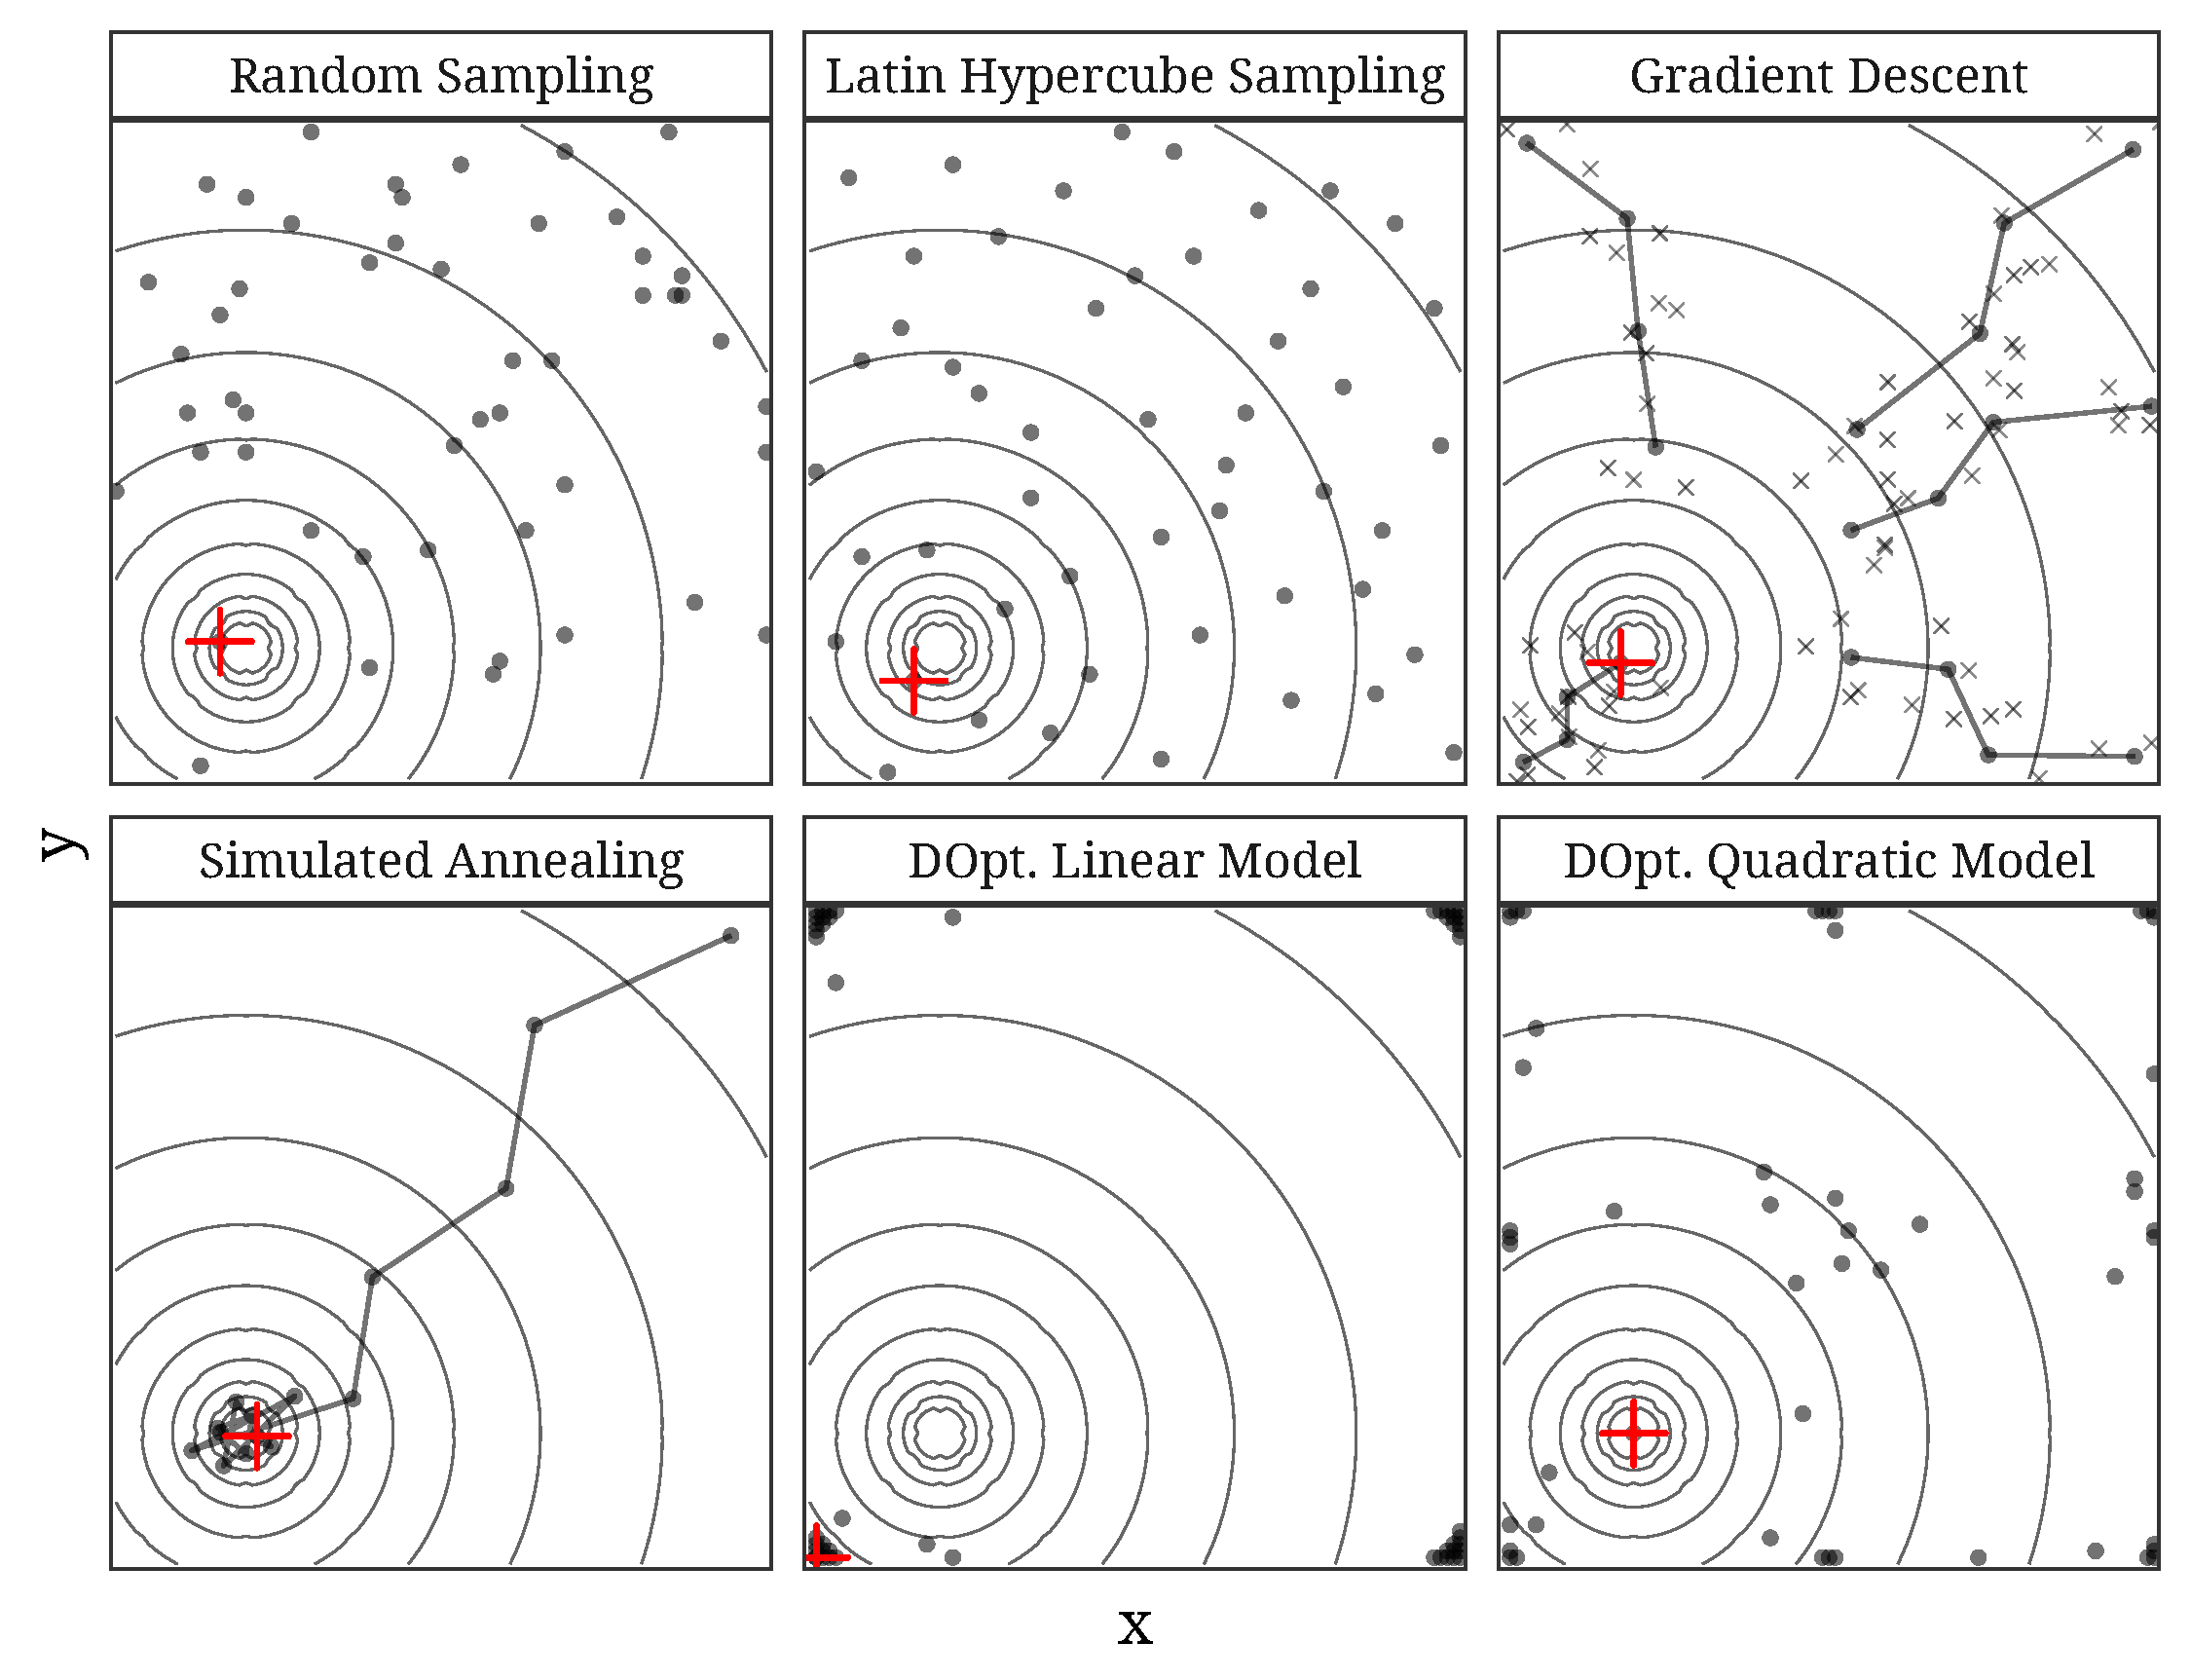
\includegraphics[width=.95\columnwidth]{./img/sampling_comparison.pdf}
\caption{Exploration of the search space defined by \(x^2 + y^2\), using a fixed budget of 50 points}
\end{figure}
\end{center}
\section{Design of Experiments}
\label{sec:org0c81bd2}
An \emph{experimental design} determines a selection of experiments whose objective
is to identify the relationships between \emph{factors} and \emph{responses}. While
factors and responses can refer to different concrete entities in other domains,
in computer experiments factors can be configuration parameters for algorithms
and compilers, for example, and responses can be the execution time or memory
consumption of a program. Each possible value of a factor is called a \emph{level}.

Experimental designs are constructed with objectives such as identifying the
most important factors and building an analytical model for the response. This
Section discusses some design construction techniques we explored and presents
the technique we selected for our approach.
\subsection{Screening}
\label{sec:org20804b7}
% latex table generated in R 3.5.1 by xtable 1.8-2 package
% Thu Oct  4 17:57:02 2018
\begin{table}[ht]
\centering
\caption{Randomized Plackett-Burman design for 12 factors}
\begingroup\small
\begin{tabular}{cccccccccccc}
  \toprule
A & B & C & D & E & F & G & H & J & K & L & Y \\
  \midrule
1 & 1 & -1 & -1 & -1 & 1 & -1 & 1 & 1 & -1 & 1 & 7.40 \\
  1 & 1 & -1 & 1 & 1 & 1 & -1 & -1 & -1 & 1 & -1 & 7.30 \\
  1 & -1 & 1 & 1 & -1 & 1 & 1 & 1 & -1 & -1 & -1 & 11.80 \\
  -1 & -1 & -1 & -1 & -1 & -1 & -1 & -1 & -1 & -1 & -1 & 5.20 \\
  1 & 1 & 1 & -1 & -1 & -1 & 1 & -1 & 1 & 1 & -1 & 9.10 \\
  1 & -1 & -1 & -1 & 1 & -1 & 1 & 1 & -1 & 1 & 1 & 9.10 \\
  -1 & -1 & 1 & -1 & 1 & 1 & -1 & 1 & 1 & 1 & -1 & 3.80 \\
  -1 & 1 & 1 & 1 & -1 & -1 & -1 & 1 & -1 & 1 & 1 & 5.10 \\
  -1 & 1 & 1 & -1 & 1 & 1 & 1 & -1 & -1 & -1 & 1 & 8.30 \\
  1 & -1 & 1 & 1 & 1 & -1 & -1 & -1 & 1 & -1 & 1 & 8.70 \\
  -1 & -1 & -1 & 1 & -1 & 1 & 1 & -1 & 1 & 1 & 1 & 8.20 \\
  -1 & 1 & -1 & 1 & 1 & -1 & 1 & 1 & 1 & -1 & -1 & 9.60 \\
   \bottomrule
\end{tabular}
\endgroup
\end{table}

\subsubsection{Analysis of Variance (ANOVA)}
\label{sec:org6e0fece}
\begin{figure}
{\normalsize
\begin{align*}
\mathbf{Y} = \bm{\beta}\mathbf{X} + \bm{\epsilon}
\end{align*}
}
\caption{Linear model assumed in main-effect analysis of screening designs}
\end{figure}
\subsection{Multi-Level Design Construction Techniques}
\label{sec:org5b55232}
The application of Design of Experiments to autotuning problems requires design
construction techniques that support factors of different types and number of
possible values. Autotuning problems typically combine factors such as binary
flags, integer and floating point numerical values, and unordered enumerations
of abstract values. Minimizing the number of experiments needed to find good
optimizations is a also a fundamental requirement since we are interested in
autotuning for scenarios with tight budget constraints.

The design construction techniques that fit these requirements are limited.
Designs that simply test all possible factor combinations, or \emph{full factorial
designs}, would provide complete information about the global minimum but are
unfeasible for most autotuning problems. In the \emph{2-level screening with random
level sampling} technique, factors with more than two unordered levels are
sampled at two random levels. This enables using small design such as the
Plackett-Burman~\cite{plackett1946design} screening design. Advantages are
the small design size and good estimation capability for main effects.
Incapability of estimating interactions is a disadvantage of this strategy, but
the main drawback is the lack of information for levels not selected in the
initial screening.

In \emph{contractive replacement}, an initial 2-level design is used to generate
mixed-level designs by re-encoding columns into a new single column representing
a multi-level factor. The contractive replacement of
Addelman-Kempthorne~\cite{addelman1961some} is a strategy of this kind.
Advantages of this technique are the small design sizes and the ability to
estimate main effects. Additionally, the contractive replacement technique
preserves orthogonality. Due to strict requirements on initial designs, not all
2-level designs can be contracted.

The \emph{direct generation} algorithm presented by Grömping and
Fontana~\cite{ulrike2018algorithm} enables the generation of multi-level
designs by solving Mixed Integer Problems (MIP). The advantages of this
technique are the direct generation of multi-level designs and a clearly defined
optimality criterion. Since this construction relies on solving carefully
formulated MIP problems, it presents strong restrictions on the size and shape
of the designs that can be generated.
\subsection{D-Optimal Designs}
\label{sec:orgfc8693c}
\emph{D-Optimal designs} are the class of designs that best fits our requirements of
supporting multi-level factors and minimizing the number of experiments. The
algorithms for constructing D-Optimal designs are relatively fast and have few
restrictions.

It is necessary to select a model that relates factors and responses to
construct a D-Optimal design. The model selection can be based on previous
experiments or on expert knowledge of the problem. Once a model is selected,
algorithmic construction is performed by searching for the set of experiments
that minimizes the \emph{D-Optimality} criterion, a measure of the \emph{variance} of the
\emph{estimators} of the \emph{regression coefficients} associated with the selected
model. This search is usually done by swapping experiments from the current
candidate set with experiments from a pool of possible experiments, according to
certain rules, until some stopping criterion is met. In the approach presented
in this paper we used Fedorov's algorithm~\cite{fedorov1972theory} for
constructing D-Optimal designs, implemented in \texttt{R} in the \texttt{AlgDesign} package.

Considering that we are going to analyze the results of an experiments plan, the
\emph{D-Efficiency} of a design is inversely proportional to the \emph{geometric mean} of
the \emph{eigenvalues} of the plan's \emph{covariance matrix}. A D-Optimal design has the
best D-Efficiency. Our current approach is based on D-Optimal designs.
\section{Applying Design of Experiments to Autotuning}
\label{sec:org2cfbaf8}
\subsection{The DLMT Strategy}
\label{sec:orgc3d017e}
\begin{center}
\begin{center}
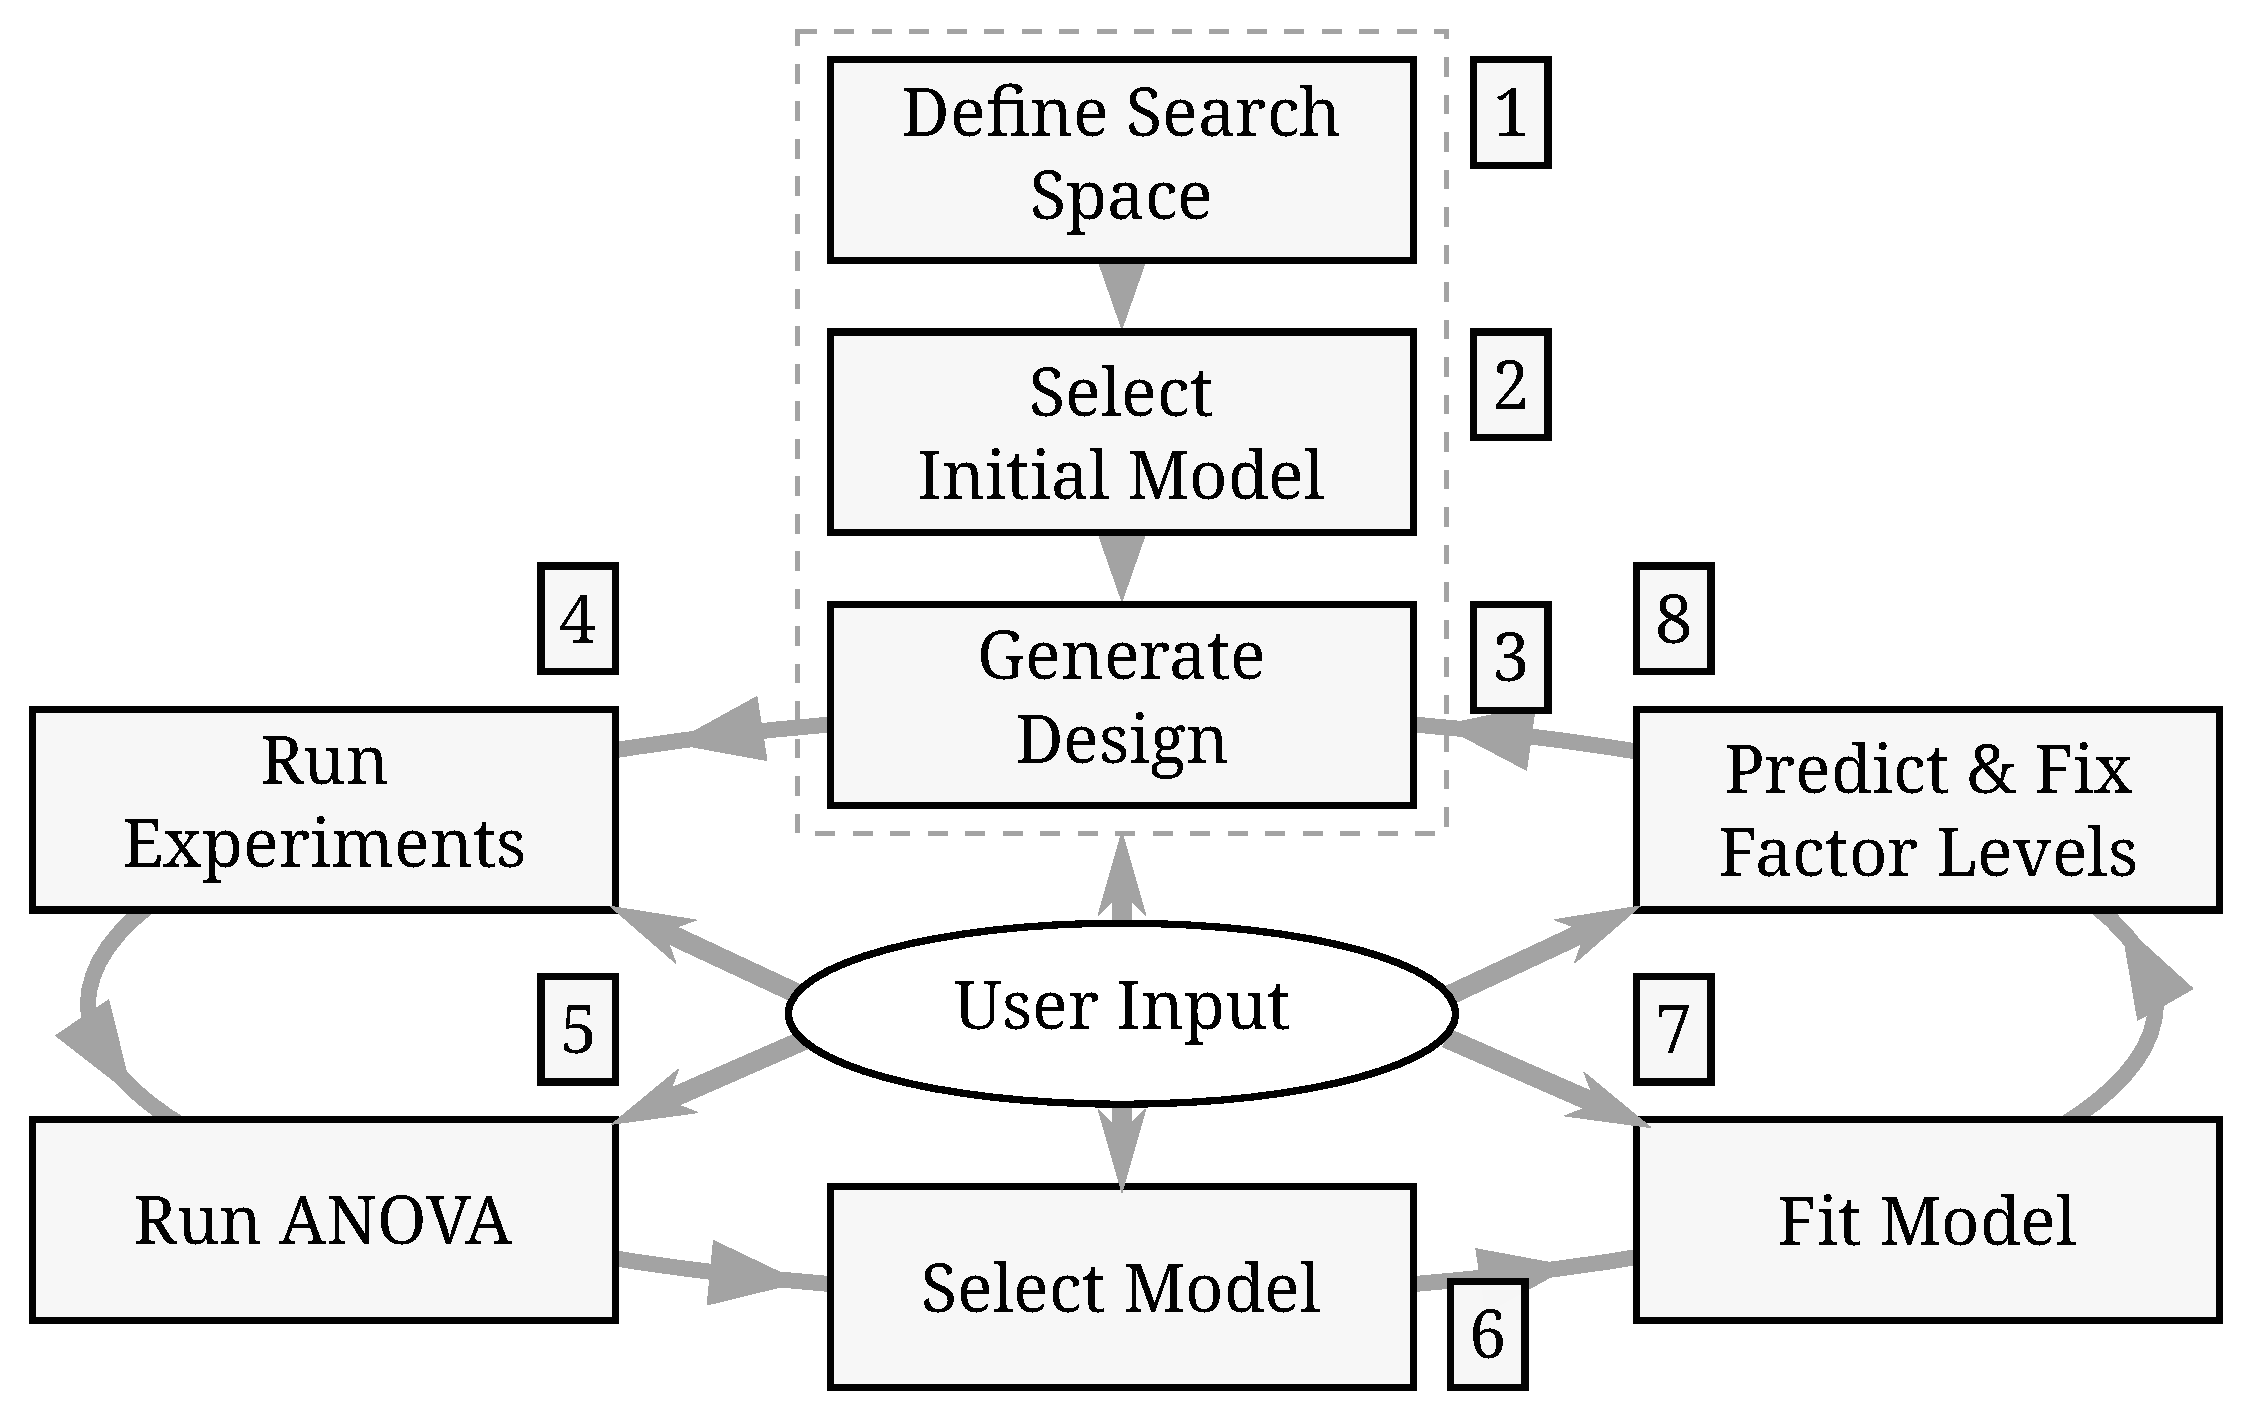
\includegraphics[width=.8\columnwidth]{./img/doe_anova_strategy.pdf}
\end{center}
\end{center}
\section{Performance Evaluation}
\label{sec:org94a595e}
\subsection{Example on a GPU Laplacian Kernel}
\label{sec:org3eed071}
\begin{figure}
{\scriptsize
\begin{align*}
\texttt{time\_per\_pixel} \thicksim & \; \texttt{y\_component\_number} + 1 / \texttt{y\_component\_number} \; + \\
& \; \texttt{vector\_length} + \texttt{lws\_y} + 1 / \texttt{lws\_y} \; + \\
& \; \texttt{load\_overlap} + \texttt{temporary\_size} \; + \\
& \; \texttt{elements\_number} + 1 / \texttt{elements\_number} \; + \\
& \; \texttt{threads\_number} + 1 /\texttt{threads\_number}
\end{align*}
}
\caption{Initial performance model used by LM and DLMT}
\end{figure}

\begin{table}[ht]
\caption{Algorithms compared in the GPU Laplacian Kernel}
\centering
\footnotesize
\begin{tabular}{ll}
\toprule
 & Algorithm\\
\midrule
RS & Random Sampling\\
LHS & Latin Hyper Square Sampling\\
GS & Greedy Search\\
GSR & Greedy Search w/ Restart\\
GA & Genetic Algorithm\\
LM & Iterative Linear Model\\
DLMT & D-Optimal Designs\\
\bottomrule
\end{tabular}
\end{table}

\subsubsection{Results}
\label{sec:orgdf0334b}
% latex table generated in R 3.5.1 by xtable 1.8-2 package
% Thu Oct  4 17:57:03 2018
\begin{table}[ht]
\centering
\caption{Slowdown and budget used by 7 optimization methods on the Laplacian Kernel, using a budget of 125 points with 1000 repetitions}
\begingroup\small
\begin{tabular}{lrrrrr}
  \toprule
 & Mean & Min. & Max. & Mean Points & Max Points \\
  \midrule
RS & 1.10 & 1.00 & 1.39 & 120.00 & 120.00 \\
  LHS & 1.17 & 1.00 & 1.52 & 98.92 & 125.00 \\
  GS & 6.46 & 1.00 & 124.76 & 22.17 & 106.00 \\
  GSR & 1.23 & 1.00 & 3.16 & 120.00 & 120.00 \\
  GA & 1.12 & 1.00 & 1.65 & 120.00 & 120.00 \\
  LM & 1.02 & 1.01 & 3.77 & 119.00 & 119.00 \\
  DLMT & 1.01 & 1.01 & 1.01 & 54.84 & 56.00 \\
   \bottomrule
\end{tabular}
\endgroup
\end{table}

\begin{center}
\begin{figure}[ht]
\centering
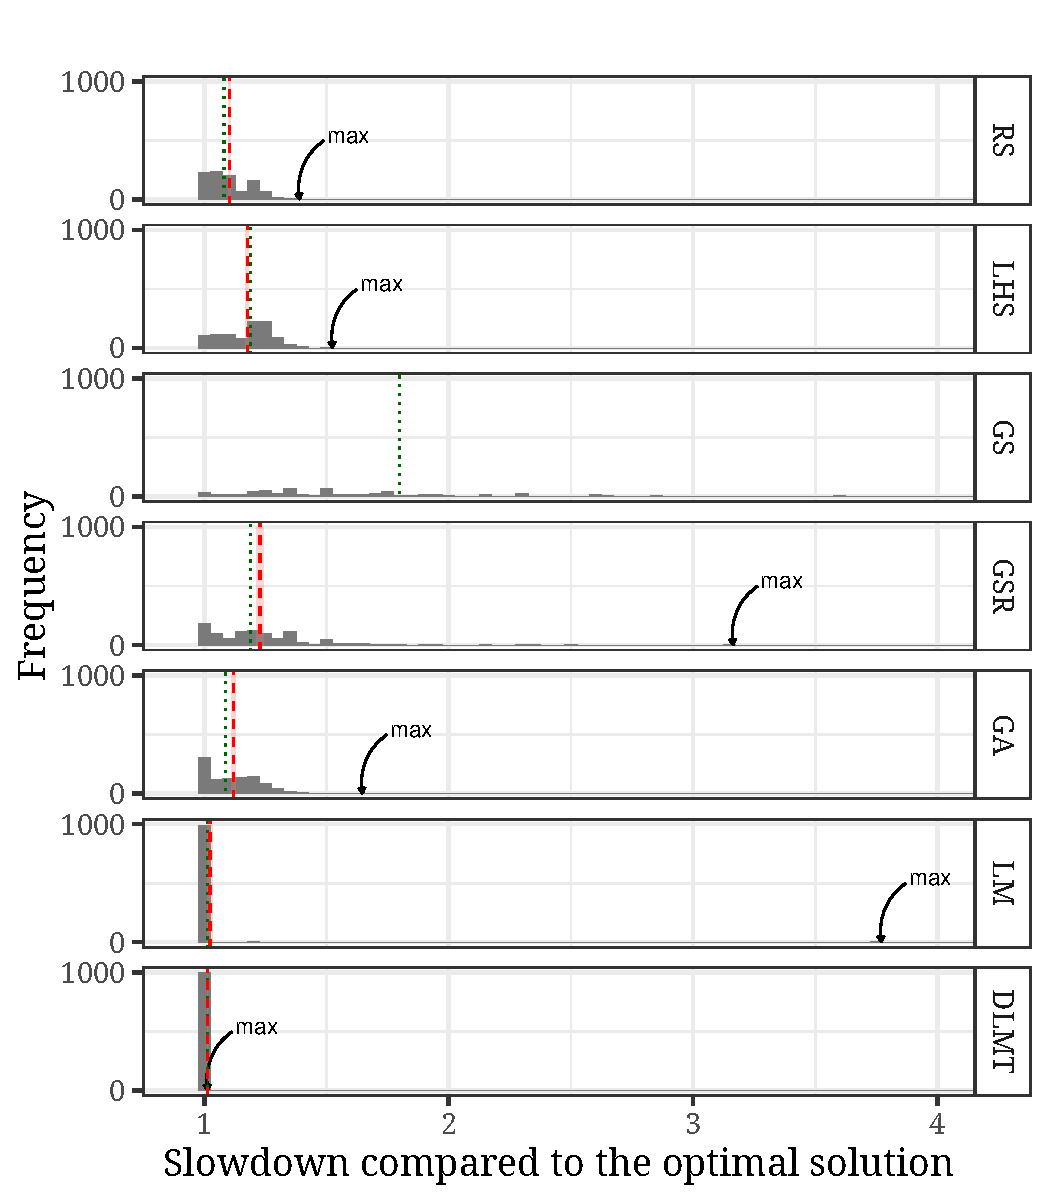
\includegraphics[width=.9\columnwidth]{./img/comparison_histogram.pdf}
\caption{Histograms of 7 optimization methods on the Laplacian Kernel, using a budget of 125 points with 1000 repetitions}
\end{figure}
\end{center}
\subsection{Results on the SPAPT Benchmark}
\label{sec:orgc020dc4}
\subsubsection{The SPAPT Benchmark}
\label{sec:orgc3c8cf3}
\begin{table}[ht]
\caption{Set of applications we used from the SPAPT benchmark}
\centering
\scriptsize
\begin{tabular}{llll}
\toprule
Kernel & Operation & Factors & Size\\
\midrule
\texttt{atax} & Matrix transp. \& vector mult. & 18 & \(2.6 \times 10^{16}\)\\
\texttt{dgemv3} & Scalar, vector \& matrix mult. & 49 & \(3.8 \times 10^{36}\)\\
\texttt{gemver} & Vector mult. \& matrix add. & 24 & \(2.6 \times 10^{22}\)\\
\texttt{gesummv} & Scalar, vector, \& matrix mult. & 11 & \(5.3 \times 10^{9}\)\\
\texttt{hessian} & Hessian computation & 9 & \(3.7 \times 10^{7}\)\\
\texttt{mm} & Matrix multiplication & 13 & \(1.2 \times 10^{12}\)\\
\texttt{mvt} & Matrix vector product \& transp. & 12 & \(1.1 \times 10^{9}\)\\
\texttt{tensor} & Tensor matrix mult. & 20 & \(1.2 \times 10^{19}\)\\
\texttt{trmm} & Triangular matrix operations & 25 & \(3.7 \times 10^{23}\)\\
\texttt{bicg} & Subkernel of BiCGStab & 13 & \(3.2 \times 10^{11}\)\\
\texttt{lu} & LU decomposition & 14 & \(9.6 \times 10^{12}\)\\
\texttt{adi} & Matrix sub., mult., \& div. & 20 & \(6.0 \times 10^{15}\)\\
\texttt{jacobi} & 1-D Jacobi computation & 11 & \(5.3 \times 10^{9}\)\\
\texttt{seidel} & Matrix factorization & 15 & \(1.3 \times 10^{14}\)\\
\texttt{stencil3d} & 3-D stencil computation & 29 & \(9.7 \times 10^{27}\)\\
\texttt{correlation} & Correlation computation & 21 & \(4.5 \times 10^{17}\)\\
\bottomrule
\end{tabular}
\end{table}
\subsubsection{Experimental Methodology}
\label{sec:orgaab9e17}
\subsubsection{Results}
\label{sec:org402fb25}
\begin{center}
\begin{figure*}[p]
\centering
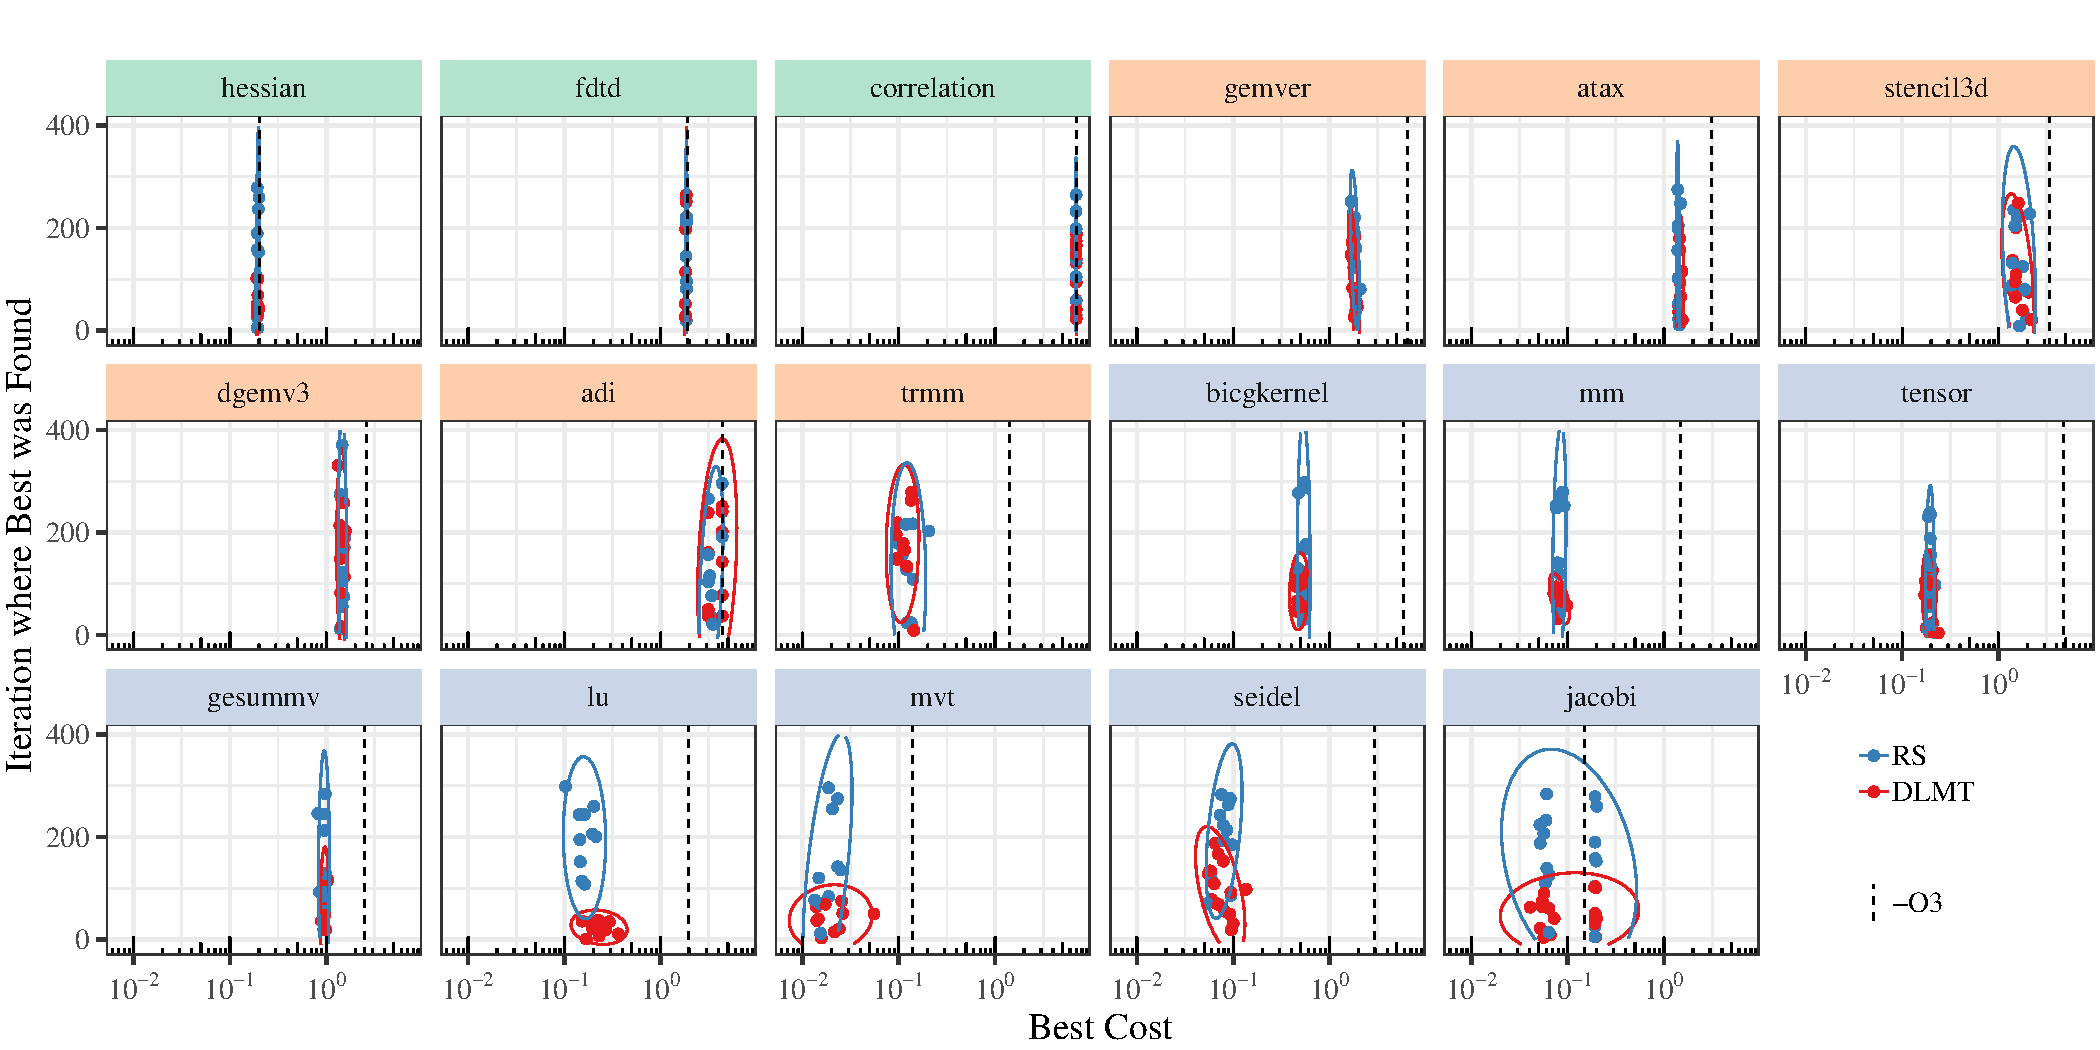
\includegraphics[width=.9\textwidth]{./img/iteration_best_comparison.pdf}
\caption{Results}
\end{figure*}
\end{center}
\clearpage
\section{Conclusion}
\label{sec:org8cea8dc}
\section*{Acknowledgment}
\label{sec:orgcbda47f}
\bibliographystyle{IEEEtran}
\bibliography{references}
\end{document}
